%%% -*-LaTeX-*-

\chapter{Evaluation}

\begin{table}[H]
\def\arraystretch{1.25}%  1 is the default, change whatever you need
\begin{tabular}{@{}l@{\hskip 12pt}l@{}}
\toprule
\textbf{CPU} & Intel Xeon E5-2450 (2.1~GHz, 2.9~GHz Turbo) \\
    & 8 cores, 2 hardware threads each \\
\textbf{RAM} & 16~GB DDR3 at 1600~MHz \\
\textbf{Network} & Mellanox MX354A ConnectX-3 Infiniband HCA (56 Gbps Full Duplex) \\
        & Connected via PCIExpress 3.0 x8 (63~Gbps Full Duplex) \\
%        & 7 Mellanox SX6036G FDR Switches \\
\textbf{Software} & CentOS 6.6, Linux 2.6.32, gcc 4.9.2, libibverbs 1.1.8, mlx4 1.0.6 \\
\bottomrule
\end{tabular}
\vspace{0.25eX}
\caption{Experimental cluster configuration.}
\label{tbl:config}
\end{table}



We explored hows the different designs trade-off database server efficiency and
performance, by building a simple model of an in-memory database system that
concentrates on data transfer rather than full query processing. In all experiments,
one node acts as a server and transmits results to 15 client nodes.
Our experiments were run on the Apt~\cite{Ricci+:OSR15} cluster of the
CloudLab~\cite{Cloudlab:URL} testbed: this testbed provides exclusive bare-metal
access to a large number of machines with RDMA-capable Infiniband NICs.
The proposed work that is pending will give more conclusive evidence for the 
Table~\ref{tbl:config} shows the Experiment Setup for the cluster where we profiled
the Mellanox Infiniband ConnectX-3 \textregistered NIC and impact of data layout and 
use of no update in place structures on transmission throughput. The cluster has 7
Mellanox SX6036G FDR switches arranged in two layers. The switching fabric is
oversubscribed and provides about 16~Gbps of bisection bandwidth per node
when congested.


\begin{figure}[t]
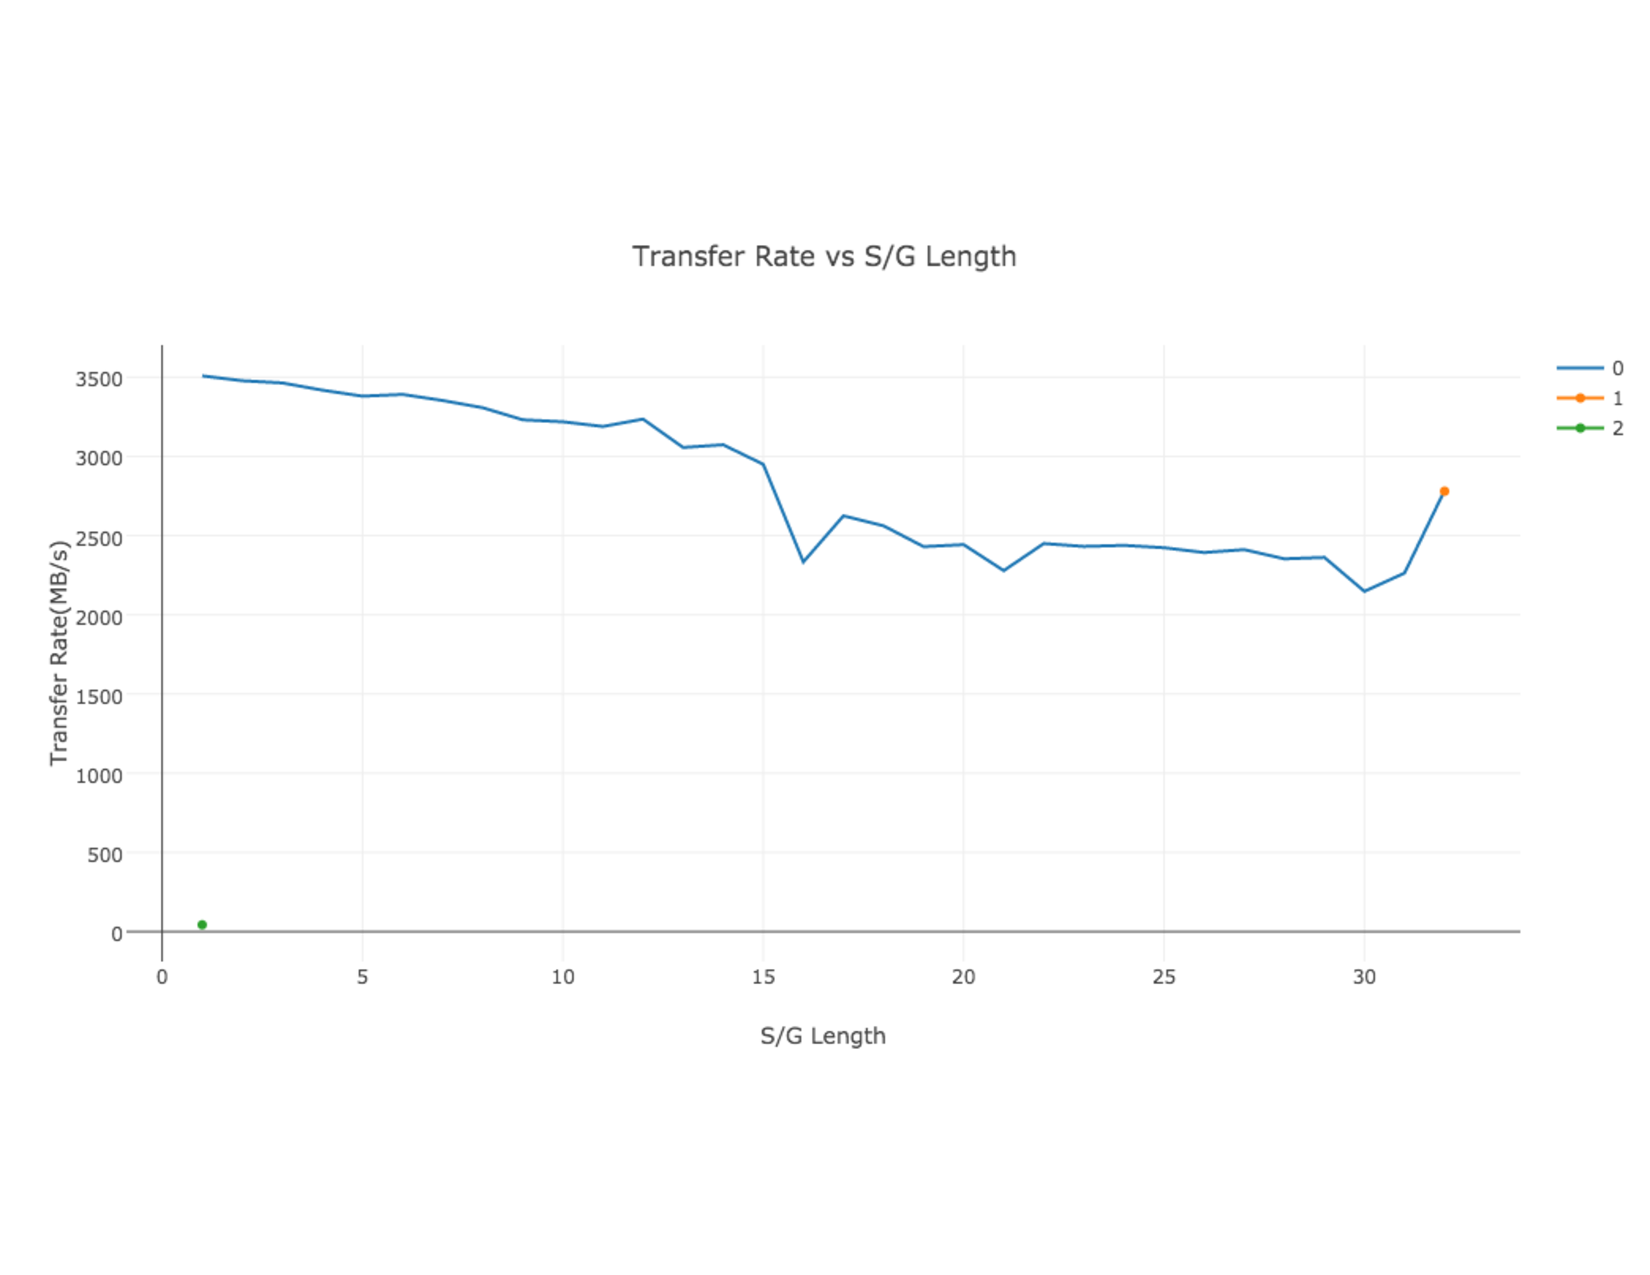
\includegraphics[width=\textwidth]{100B_transrate.pdf}
\caption{Transmission rate for 100 B records over different RDMA verbs and 
varying S/G lengths.}
\label{fig:100B_transrate}
\end{figure}

\begin{figure}[H]
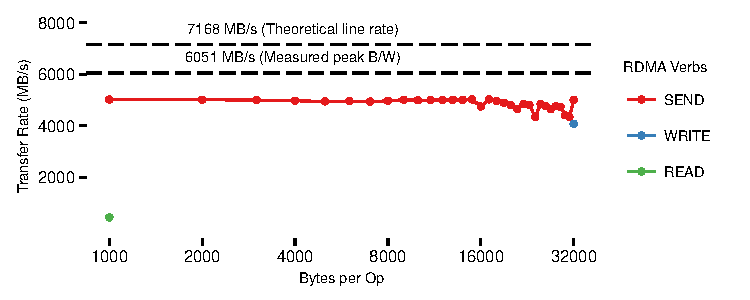
\includegraphics[width=\textwidth]{fig-1000B-RDMAverbs}
\caption{Transmission rate for 1000 B records over different RDMA verbs and 
varying S/G lengths.}
\label{fig:1000B_transrate}
\end{figure}


\section{RDMA modes}
We started out by getting measurements of transmission speeds using RDMA Reads.
We implemented rdma operations using infinibands ib verbs library. We implemented 
RDMA reads and write as op codes on the \cpp{ibv_send_wr} request which 
transmit data as \cpp{ibv_post_send} and also tried to measure the transmit
performance while using zero copy using \cpp{IBV_WR_SEND} as the operation.
We found that send operations can transmit multiple transmit buffer
It became evident quickly that one sided RDMA reads are not well positioned to 
take advantage of the zero copy paradigm since it only supports a remote read 
from a given location from the source. The rest of the experiments concerning
the impacts of NIC's impact on data layout were all done with send as the primary
operation. 


Figure~\ref{fig:100B_transrate} shows a comparison of transmission
peformance of various verbs transmitting 100 Byte records varying the number of records
that could be transmitted at a time for various operations.The green dot shows
the performance for RDMA reads which is also unfair
since RDMA reads can only transmit a single record at a time. The yellow dot
shows RDMA write performance. The modes shown was an enum of the format 
\cpp{enum Mode \{ MODE_SEND, MODE_WRITE, MODE_READ\}} and infiniband 
\cpp{<infiniband/verbs.h>} verbs library provides the  The record sizes were 
also an interesting measure to arrive at. It was obvious even from an earlier stage
that higher data sizes such as shown in Figure~\ref{fig:1000B_transrate} almost 
always results in better throughput measurements. In the world of In-memory databases,
there is an argument to be made that record sizes will be getting smaller since 
database designers can aggresively normalise and this has proven increasingly to
the liking of companies that manage large volumes of data in memory~\cite{fb-memcache,fb-workload}.


\section{Paging}
All our experiments transmit from a large region of memory backed by 4~KB pages
that contains all of the records. The region is also
registered with the NIC, which has to do virtual-to-physical address
translation to DMA records for transmission.
In some cases, using 1~GB hugepages reduces translation look aside buffer
(TLB) misses. We have realised that the NIC can benefit from
hugepages as well, since large page tables can result in additional
DMA operations to host memory during address translation~\cite{farm,rdma}. For
our experiments, the reach of the NIC's virtual-to-physical mapping is
sufficient, and hugepages have no impact on the results.


\section{Preliminary Results}
Pure comparison of Zero Copy vs Copy Out for efficient transmission of heavy range query
results that improves throughput by 1.7$\times$ (from 3.4~GB/s to 5.7~GB/s) and
reduces CPU overhead by 75\% compared to fully scattered zero-copy by relaxing
the structure of the results that clients receive.  We start with an
overview of related work in this space, then describe a modern kernel-bypass NIC
and the Bw-Tree. We continue with a set of microbenchmarks and draw
conclusions for data structure/networking layer co-design.

